\begin{figure}[ht]
   \centering
   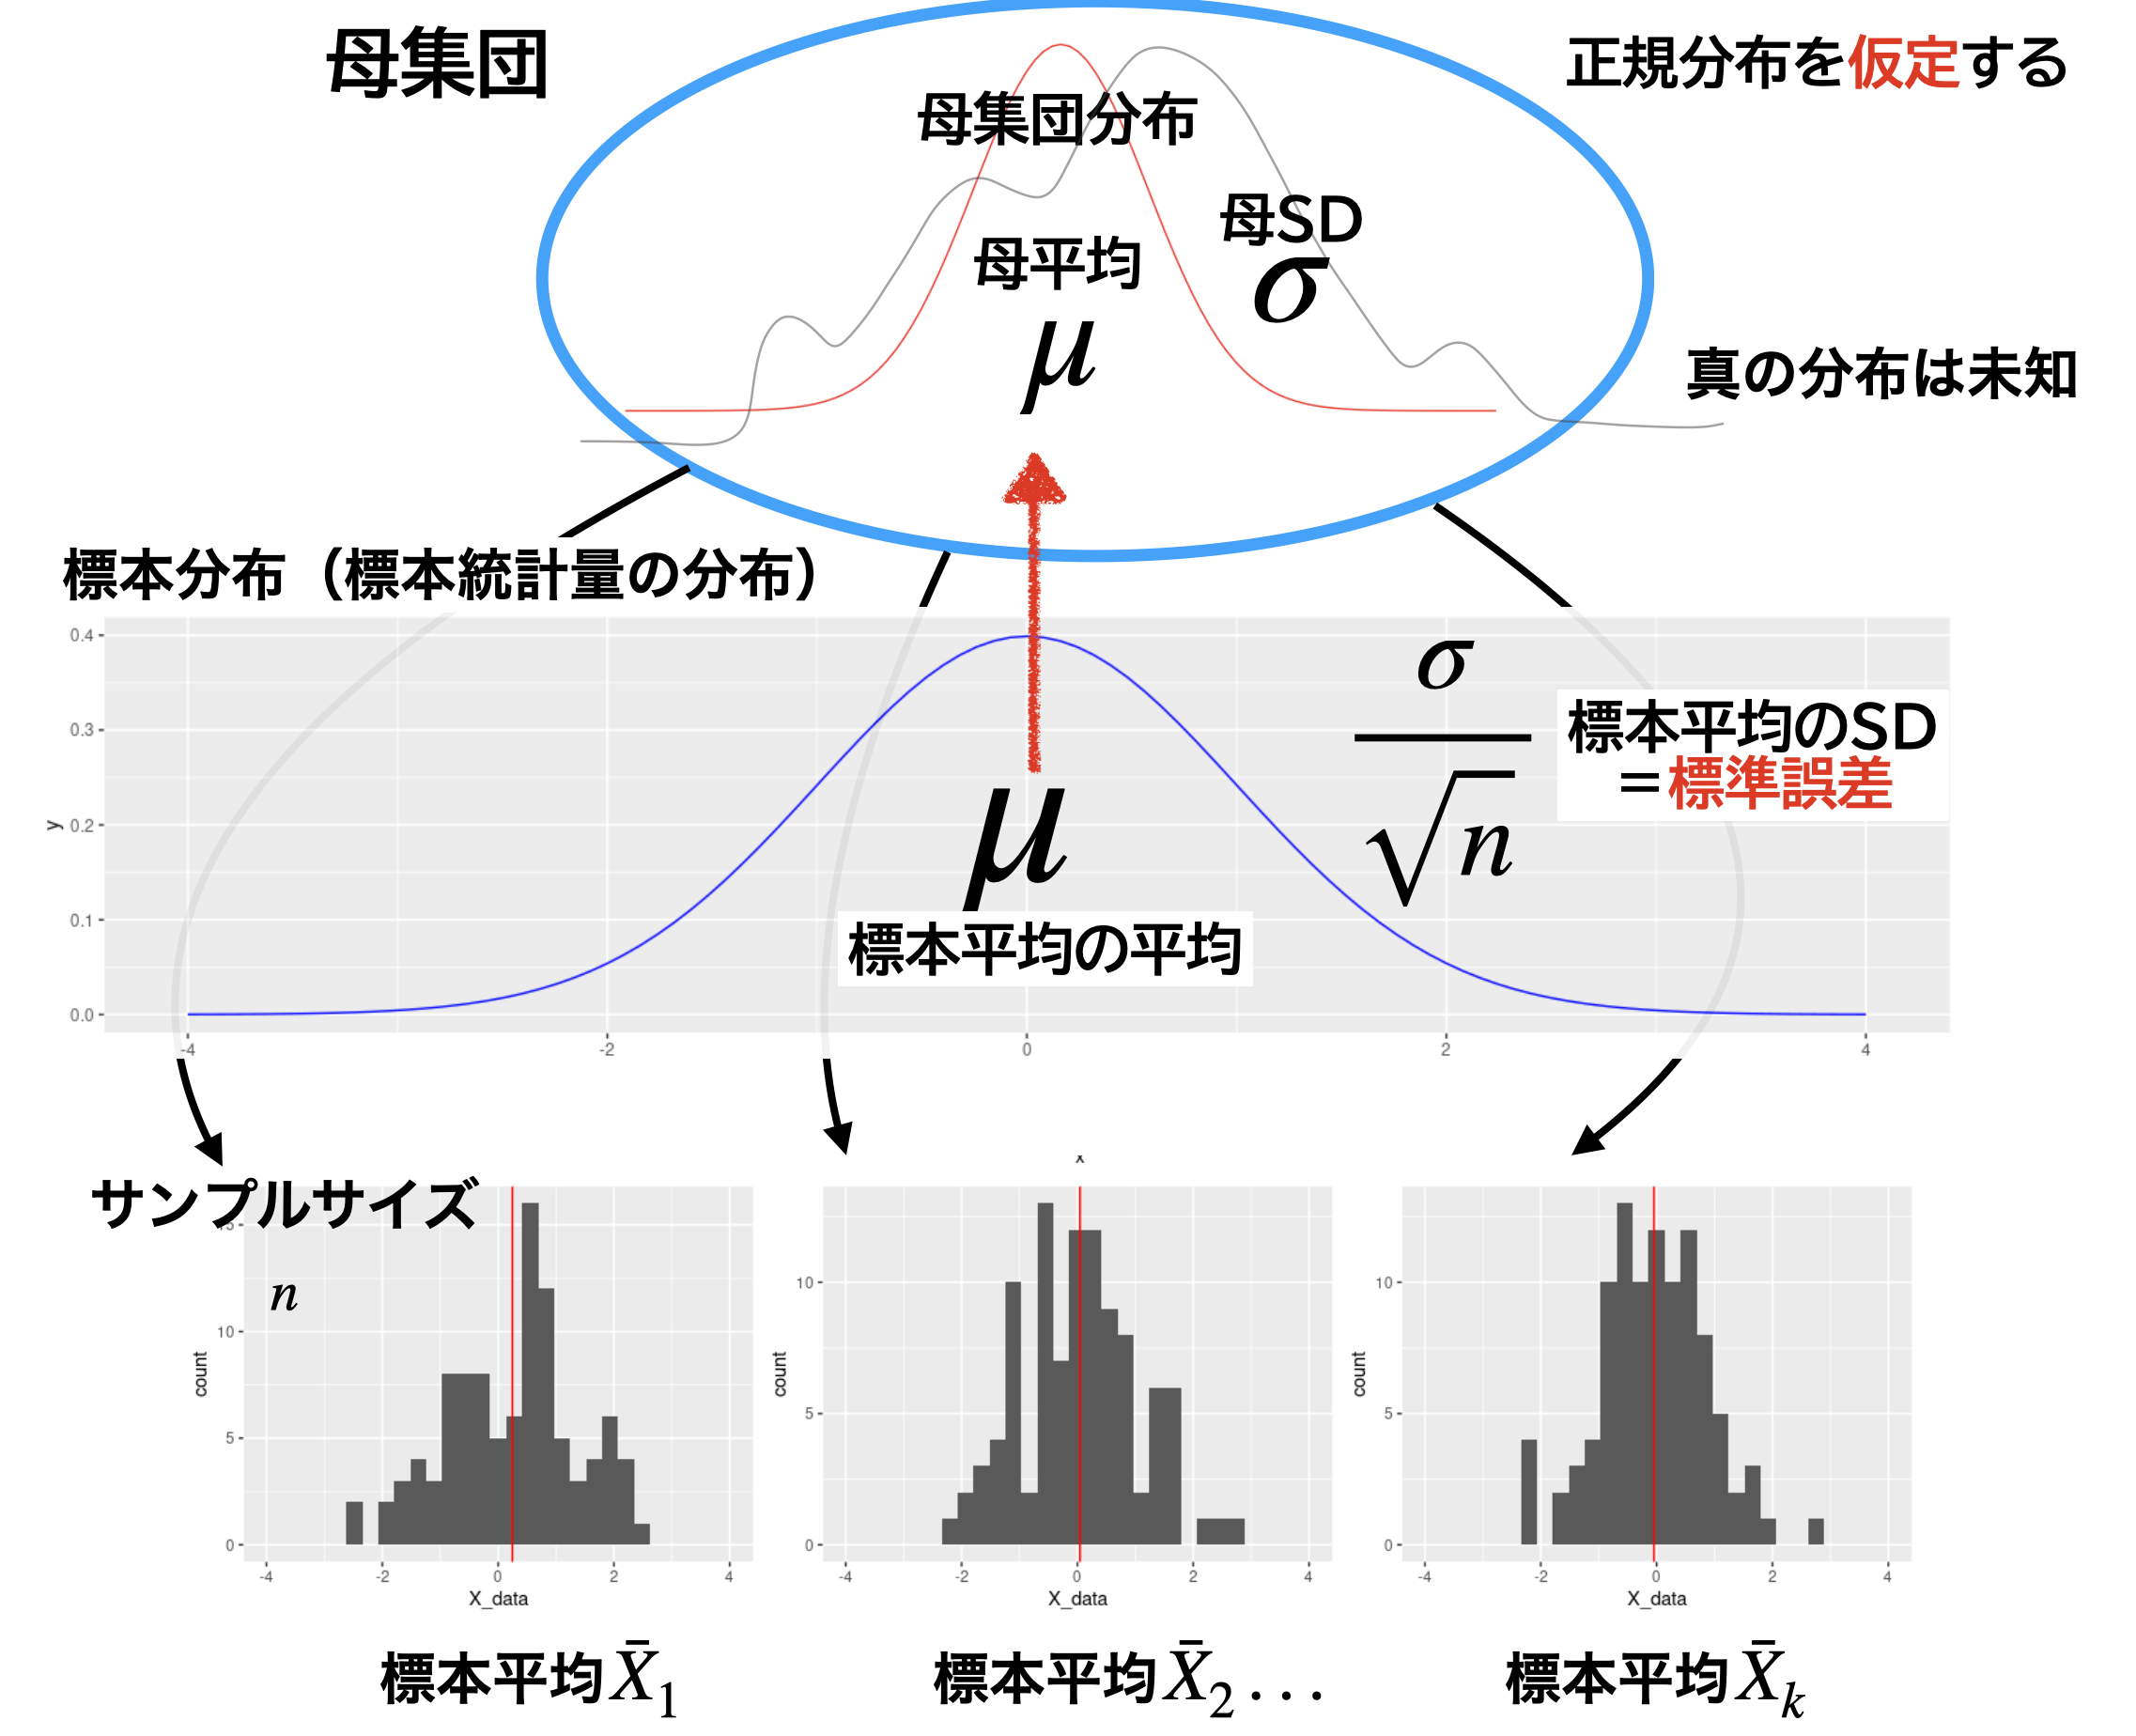
\includegraphics[keepaspectratio,height=0.6\linewidth]{../images/16_inference/slide16_03.png}
   \caption{Sample, sample statistics, sample distribution, and statistical inference. Obtain a sample of size $n$ from a population. Each data point (person figure in sample 1) is captured within the framework of the population and sample. Sample statistics yield different values each time a sample is taken ($1, 2,\ldots, k$, where $k$ is the sample size), but follows the sample distribution. The expected value of the sample distribution is equal to the population mean, and the accuracy of a sample mean can be evaluated by the standard error.}
   \label{fig::16_05}
\end{figure}
